\section{Motivation}
\label{sec:motivation}
In this section, we first motivate our work by showing how a model can be compiled in different ways
and subsequently, show the drastic performance difference across these variants for real benchmarks.

\subsection{Motivating Example}
\begin{figure}[htb]
  \centering
  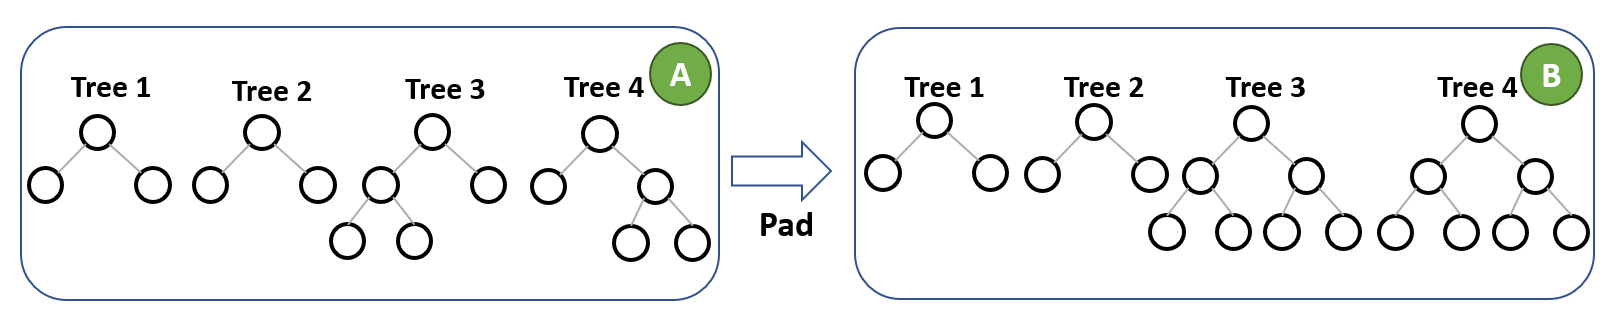
\includegraphics[width=\linewidth]{figures/HIR.PNG}
  \caption{The representation of a model in high-level IR and the model 
  after trees are padded and reordered.\TODO{drop reorder, make 1,2 depth 1 and 3,4 depth 2.} }
  \label{Fig:HIRExample}
\end{figure}

Consider a model with four trees, two 
trees of depth 1 and two of depth 2 (Figure \ref{Fig:HIRExample}).
% We use this model as our running example throughout this section.
We first describe a simple schedule that processes one tree at a time 
for all input rows. The scheduling constructs are fairly intuitive. We 
defer a detailed explanation of the scheduling language to Section~\ref{sec:scheduling}. 
The loop over the trees is split into two -- one that
iterates over the first two trees (Trees 1 and 2 with depth 1) and 
the second that iterates over the last two trees (Trees 3 and 4 with
depth 2). Straightforward traversal of trees requires a \op{while} loop
and involves branching to check if a leaf has been reached. 
One way to avoid this as done in this schedule is to unroll the 
tree walks for each tree. 
When the schedule specifies that the tree walks should be unrolled, 
\Treebeard{} pads the trees so that all leaves are at the same depth (the padded trees are also shown in Figure~\ref{Fig:HIRExample}).

\begin{lstlisting}[style=c++]
  reorder(tree, batch)
  // Fiss tree loop so trees with equal depth 
  // are processed together  
  split(tree, t_depth1, t_depth2, 2)
  // Unroll the tree walks
  unrollWalk(t_depth1, 1)
  unrollWalk(t_depth2, 2)
\end{lstlisting}
The concrete implementation of this schedule (in \Treebeard{}'s IRs) 
is as follows.
\begin{lstlisting}[style=c++]
  model = ensemble(...)
  for t_depth1 = 0 to 2 step 1 {
    T = getTree(ensemble, t_depth1)
    for batch = 0 to BATCH_SIZE step 1 {
      treePred = walkDecisionTree(T, 
                    input[batch]) <unrollDepth = 1>
      reduce(result[batch], treePred)
    }
  }
  for t_depth2 = 2 to 4 step 1 {
    T = getTree(ensemble, t_depth2)
    for batch = 0 to BATCH_SIZE step 1 {
      treePred = walkDecisionTree(T,
                    input[batch]) <unrollDepth = 2>
      reduce(result[batch], treePred) <'+', 0.0>
    }
  }
\end{lstlisting}
This schedule is ideally suited for a single-core CPU. It maximizes 
the reuse of trees in the L1 cache. However, it doesn't exploit  
any parallelism. 
%% RG, 
%%  and is therefore ill-suited for parallel processors.
% Further, the \op{batch} for loop can be tiled to get locality benefits. 

One form of parallelism that can be exploited is to process rows in 
parallel. 
%% RG:
While this may work for multi-core CPUs\footnote{As we report in Section~\ref{sec:results}, other ways to parallelize can benefit inference on CPUs as well.}, with massively parallel processors like GPUs,
 this strategy may not yield sufficient parallel work. To expose more parallelism, 
we can additionally parallelize across trees as done in the schedule below. 
%% RG:
% With GPUs, the performance of generated code would also vary with the 
% kernel configuration, which specifies the number of thread blocks\footnote{We 
% use NVIDIA CUDA terminology in the discussion, but as we demonstrate in 
% Section~\ref{sec:results}, our framework can generate code for AMD GPUs as well.}, 
% the size of thread blocks and so on. 
% A possible strategy to accomplish this is encoded in the following schedule.
\begin{lstlisting}[style=c++]
  // Split the trees into two sets
  tile(tree, t0, t1, 2)
  reorder(batch, t1, t0)
  // Fiss loop so that trees with equal 
  // depth are processed together
  split(t0, t0_depth1, t0_depth2, 2)
  unrollWalk(t0_depth1, 1)
  unrollWalk(t0_depth2, 2)
  // Configure the GPU kernel dimensions
  gpuDimension(batch, grid.x)
  gpuDimension(t1, block.x)
\end{lstlisting}
This schedule generates an inference function that runs on the GPU. 
The inference routine processes one input row per thread block (since the \op{batch}
loop is mapped directly to \op{grid.x}).
It also splits the trees into two sets by tiling the \op{tree} loop.
Each of the two sets is processed in parallel. We unroll the tree walks 
for each tree. The IR generated is as follows. 
\begin{lstlisting}[style=c++]
  model = ensemble(...)
  par.for batch = 0 to BATCH_SIZE step 1 <grid.x> {
    par.for t1 = 0 to 2 step 1 <block.x> {
      for t0_depth1 = 0 to 2 step 2 {
        T = getTree(ensemble, t0_depth1 + t1)
        treePred = walkDecisionTree(T, 
                        input[batch]) <unrollDepth = 1>
        reduce(result[batch], treePred)
      }
      for t0_depth2 = 2 to 4 step 2 {
        T = getTree(ensemble, t0_depth2 + t1)
        treePred = walkDecisionTree(T,
                        input[batch]) <unrollDepth = 2>
        reduce(result[batch], treePred) <'+', 0.0>
      }
    }
  }
\end{lstlisting}

% In the case of this schedule, the \op{reduce}
% operation needs special consideration.  
% %% RG
% %% to correctly generate code for this schedule, the compiler needs 
% To generate the correct code for this schedule, the compiler needs to determine
% the required synchronization and temporary storage for reductions 
% given the parallelization strategy specified. In the given example, it 
% has to identify that parallel iterations of the \op{t1} 
% loop accumulate into the same element of the \op{result} array.
% One possible solution is to rewrite the reduction so that each parallel 
% iteration accumulates into a different array element by introducing 
% a temporary buffer (\op{temp}) as follows.
% \begin{lstlisting}[style=c++]
%   float temp[2][BATCH_SIZE]
%   model = ensemble(...)
%   par.for batch = 0 to BATCH_SIZE step 1 <grid.x> {
%     par.for t1 = 0 to 2 step 1 <block.x> {
%       for t0_depth1 = 0 to 2 step 2 {
%         T = getTree(ensemble, t0_depth1 + t1)
%         treePred = walkDecisionTree(T, 
%                       input[batch]) <unrollDepth = 1>
%         reduce(temp[t1][batch], treePred)
%       }
%       for t0_depth2 = 2 to 4 step 2 {
%         T = getTree(ensemble, t0_depth2 + t1)
%         treePred = walkDecisionTree(T,
%                       input[batch]) <unrollDepth = 2>
%         reduce(temp[t1][batch], treePred) <'+', 0.0>
%       }
%     }
%     result[batch] = reduce_dimension(temp[:][batch], 0)
%   }
% \end{lstlisting}
% Here, partial results are accumulated into \op{temp} and then
% reduced across the \op{t1} dimension to get the final result.
Note that while unrolling helps avoid branching, it likely increases 
the total amount of computation. Another option is to not unroll 
and let the GPU manage the branching. The schedules with and 
without unrolling place different constraints on the target processor,
and the best choice depends on the characteristics of the model
and micro-architectural features like register file size, handling 
of branch divergence etc.~\cite{FungMicro11, SomethingElse}.

% As is evident from these examples, it is possible to optimize 
% the inference routine in different ways. Also, the structure of the loop 
% nest in the inference routine can get quite complex even 
% for simple schedules. Writing these routines by hand 
% is error-prone and time-consuming.  
% %% RG 
% %% We beleive 
% Hence designing a 
% scheduling language to encapsulate these strategies and a principled code 
% generator to automatically generate code guided by the schedule is the 
% best approach. We promote such an approach in this paper.

\subsection{Performance of Different Schedules} 
\begin{figure}[htb]
  \begin{subfigure}[t]{.45\linewidth}
    \vspace{0pt}
    \centering
    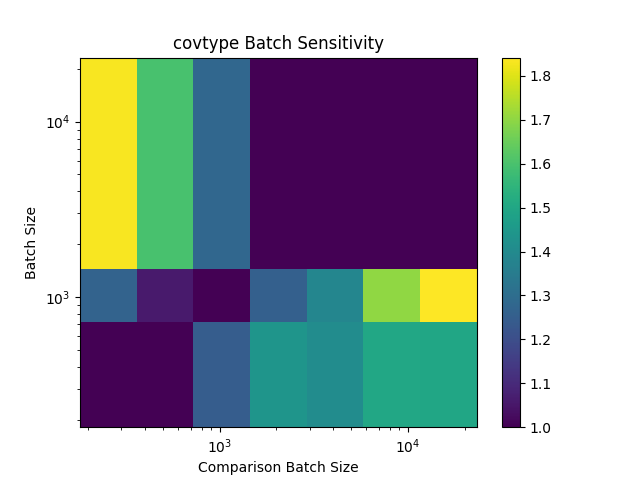
\includegraphics[width=\linewidth]{figures/batch_sensitivity_covtype.png}
    \vspace{2pt}
    \caption{\label{fig:sensitivitya}\op{covtype} batch sensitivity}
  \end{subfigure}\hfill
  \begin{subfigure}[t]{.52\linewidth}
    \vspace{0pt}
    \centering
    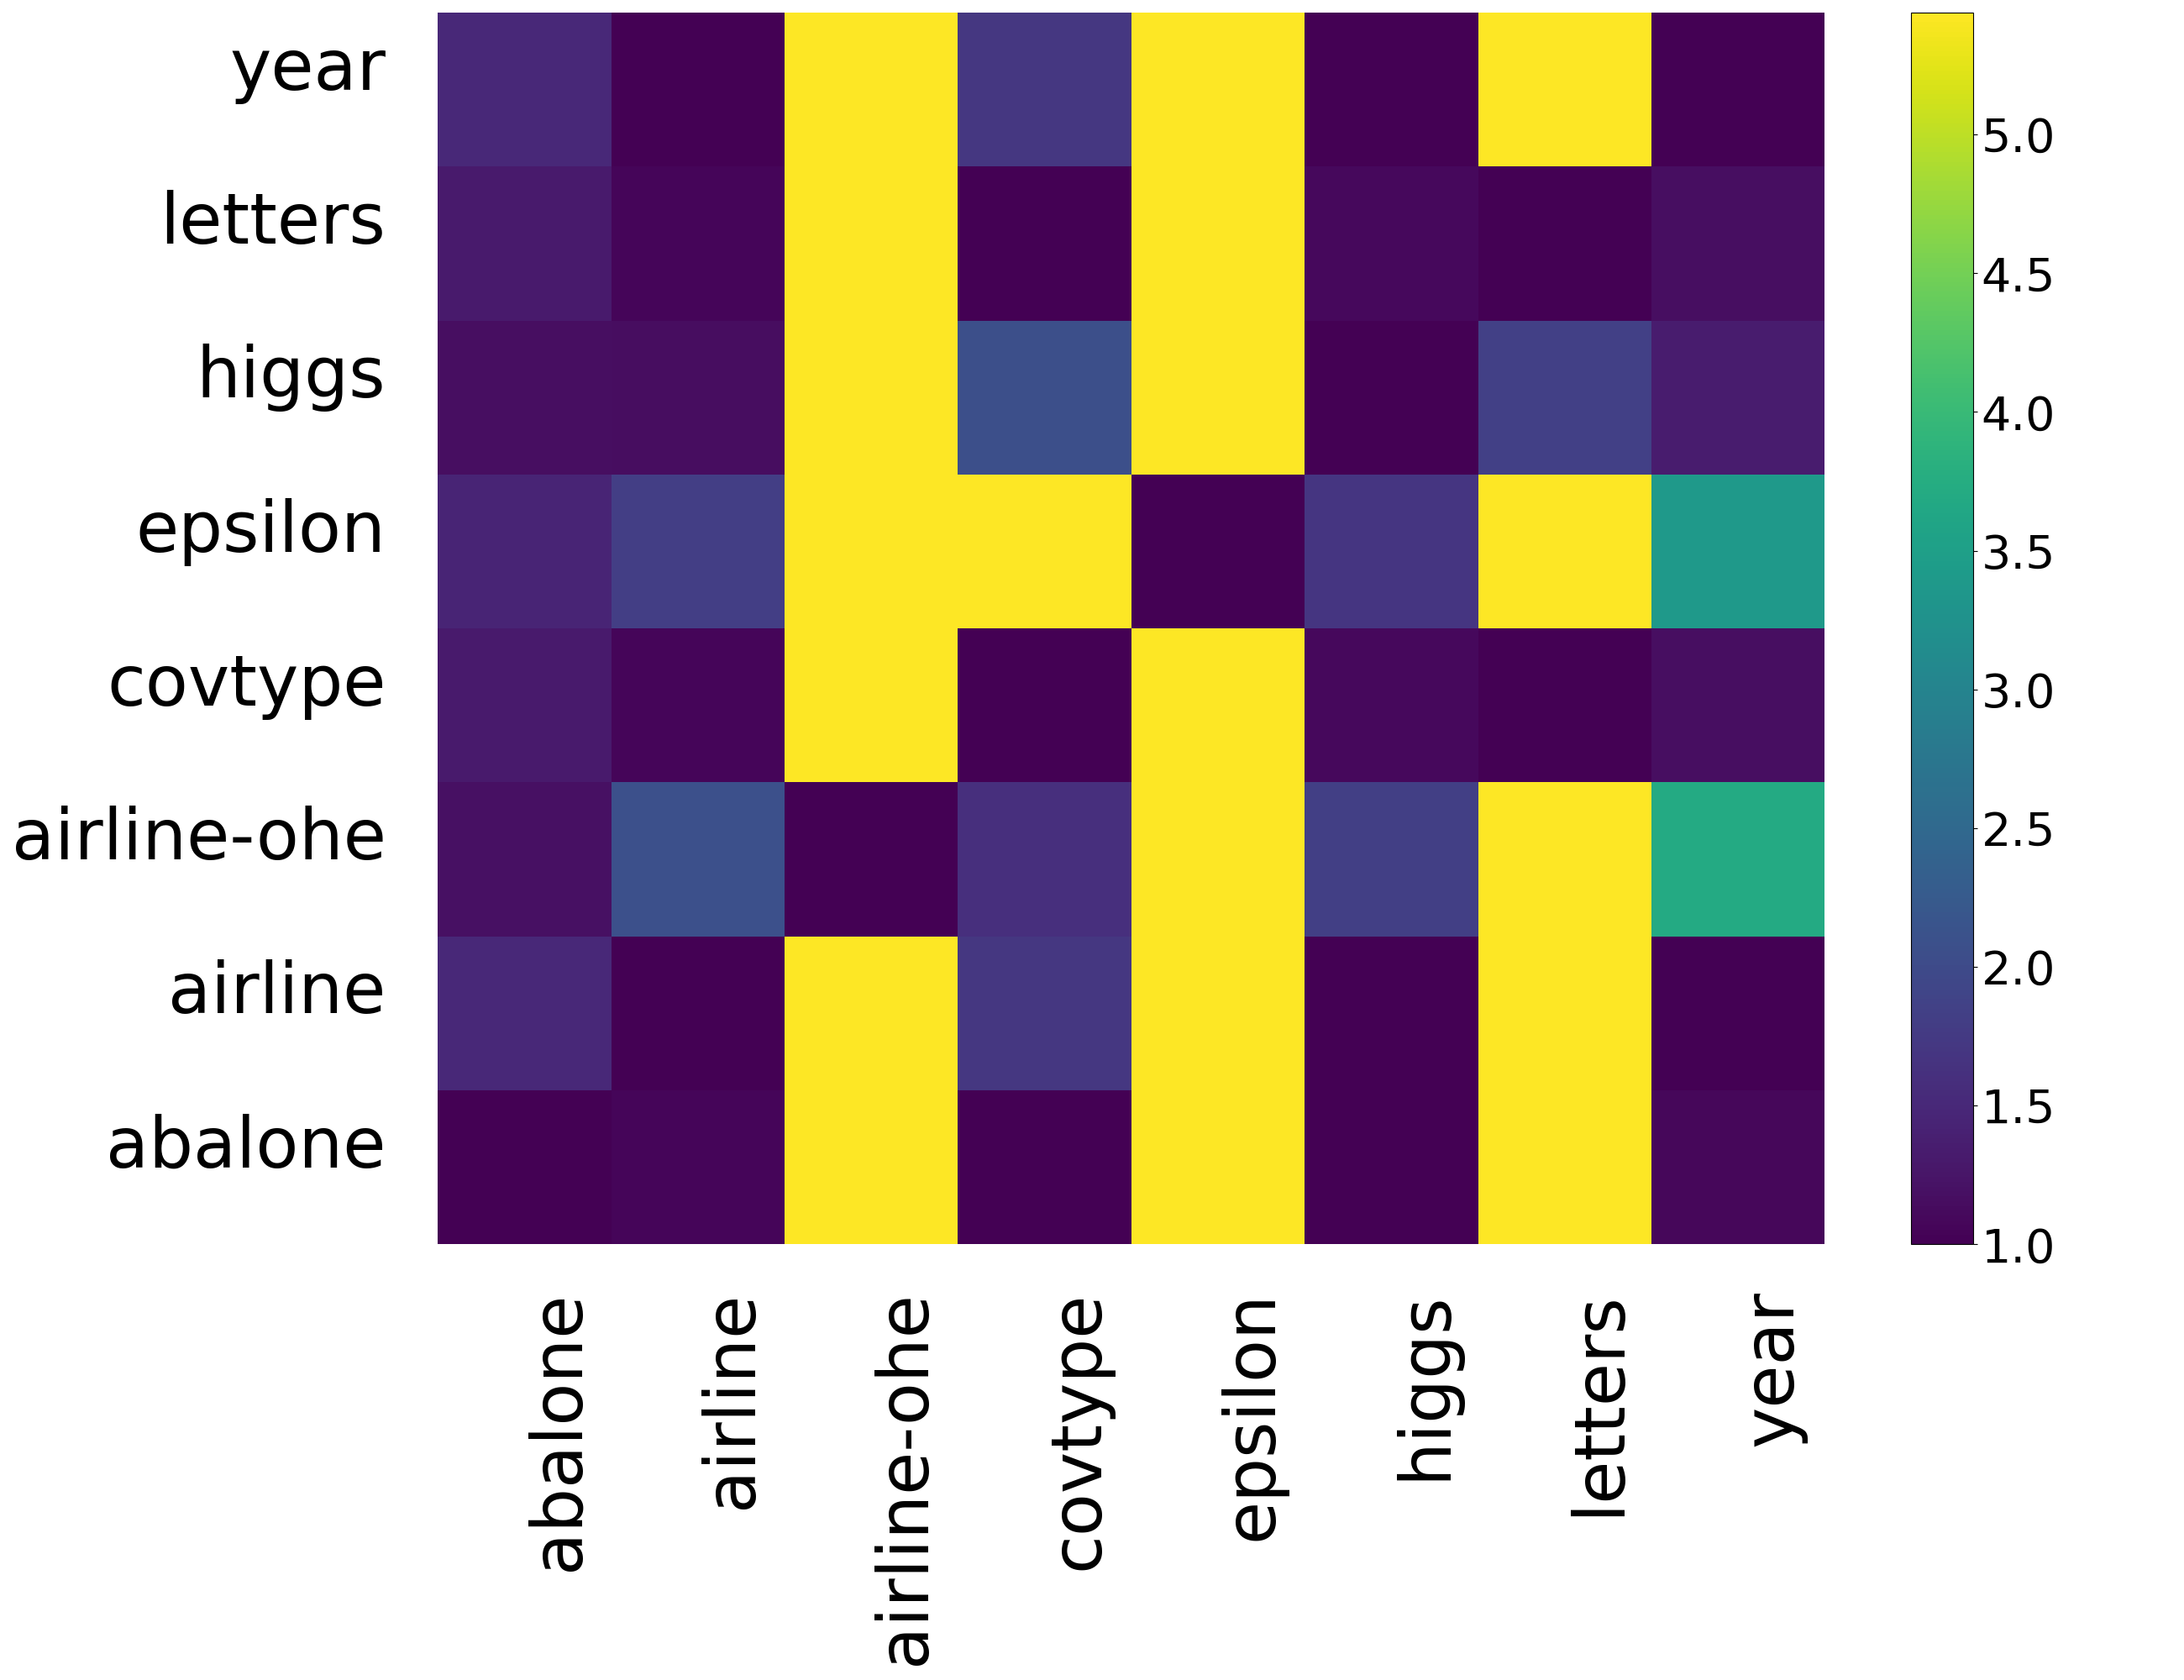
\includegraphics[width=\linewidth]{figures/model_sensitivity_4096.png}
    \caption{\label{fig:sensitivityb}Model sensitivity at batch size 4096}
  \end{subfigure}
  \caption{Batch and model sensitivity plots. Each point shows the slowdown when the best schedule for the x-axis batch size (model) is used for the y-axis batch size (model).}
\end{figure}

% \begin{figure}[htb]
%   \begin{minipage}[t]{.475\linewidth}
%     \subcaptionbox*{}{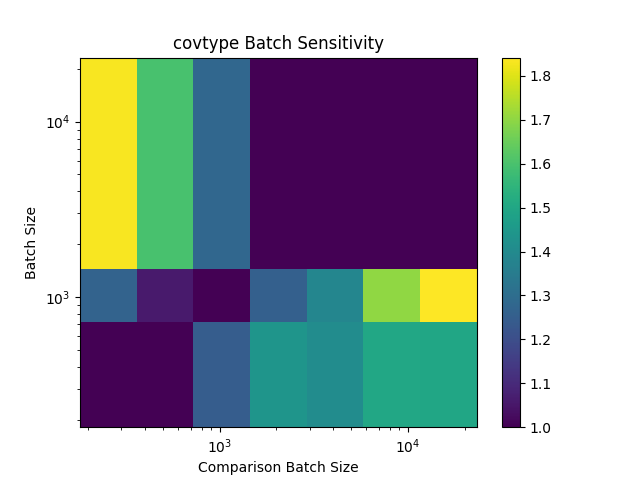
\includegraphics[width=\linewidth]{figures/batch_sensitivity_covtype.png}}
%     \caption{\label{fig:sensitivitya}Batch sensitivity for \op{covtype}}
%   \end{minipage}
%   \begin{minipage}[t]{.475\linewidth}
%     \subcaptionbox*{}{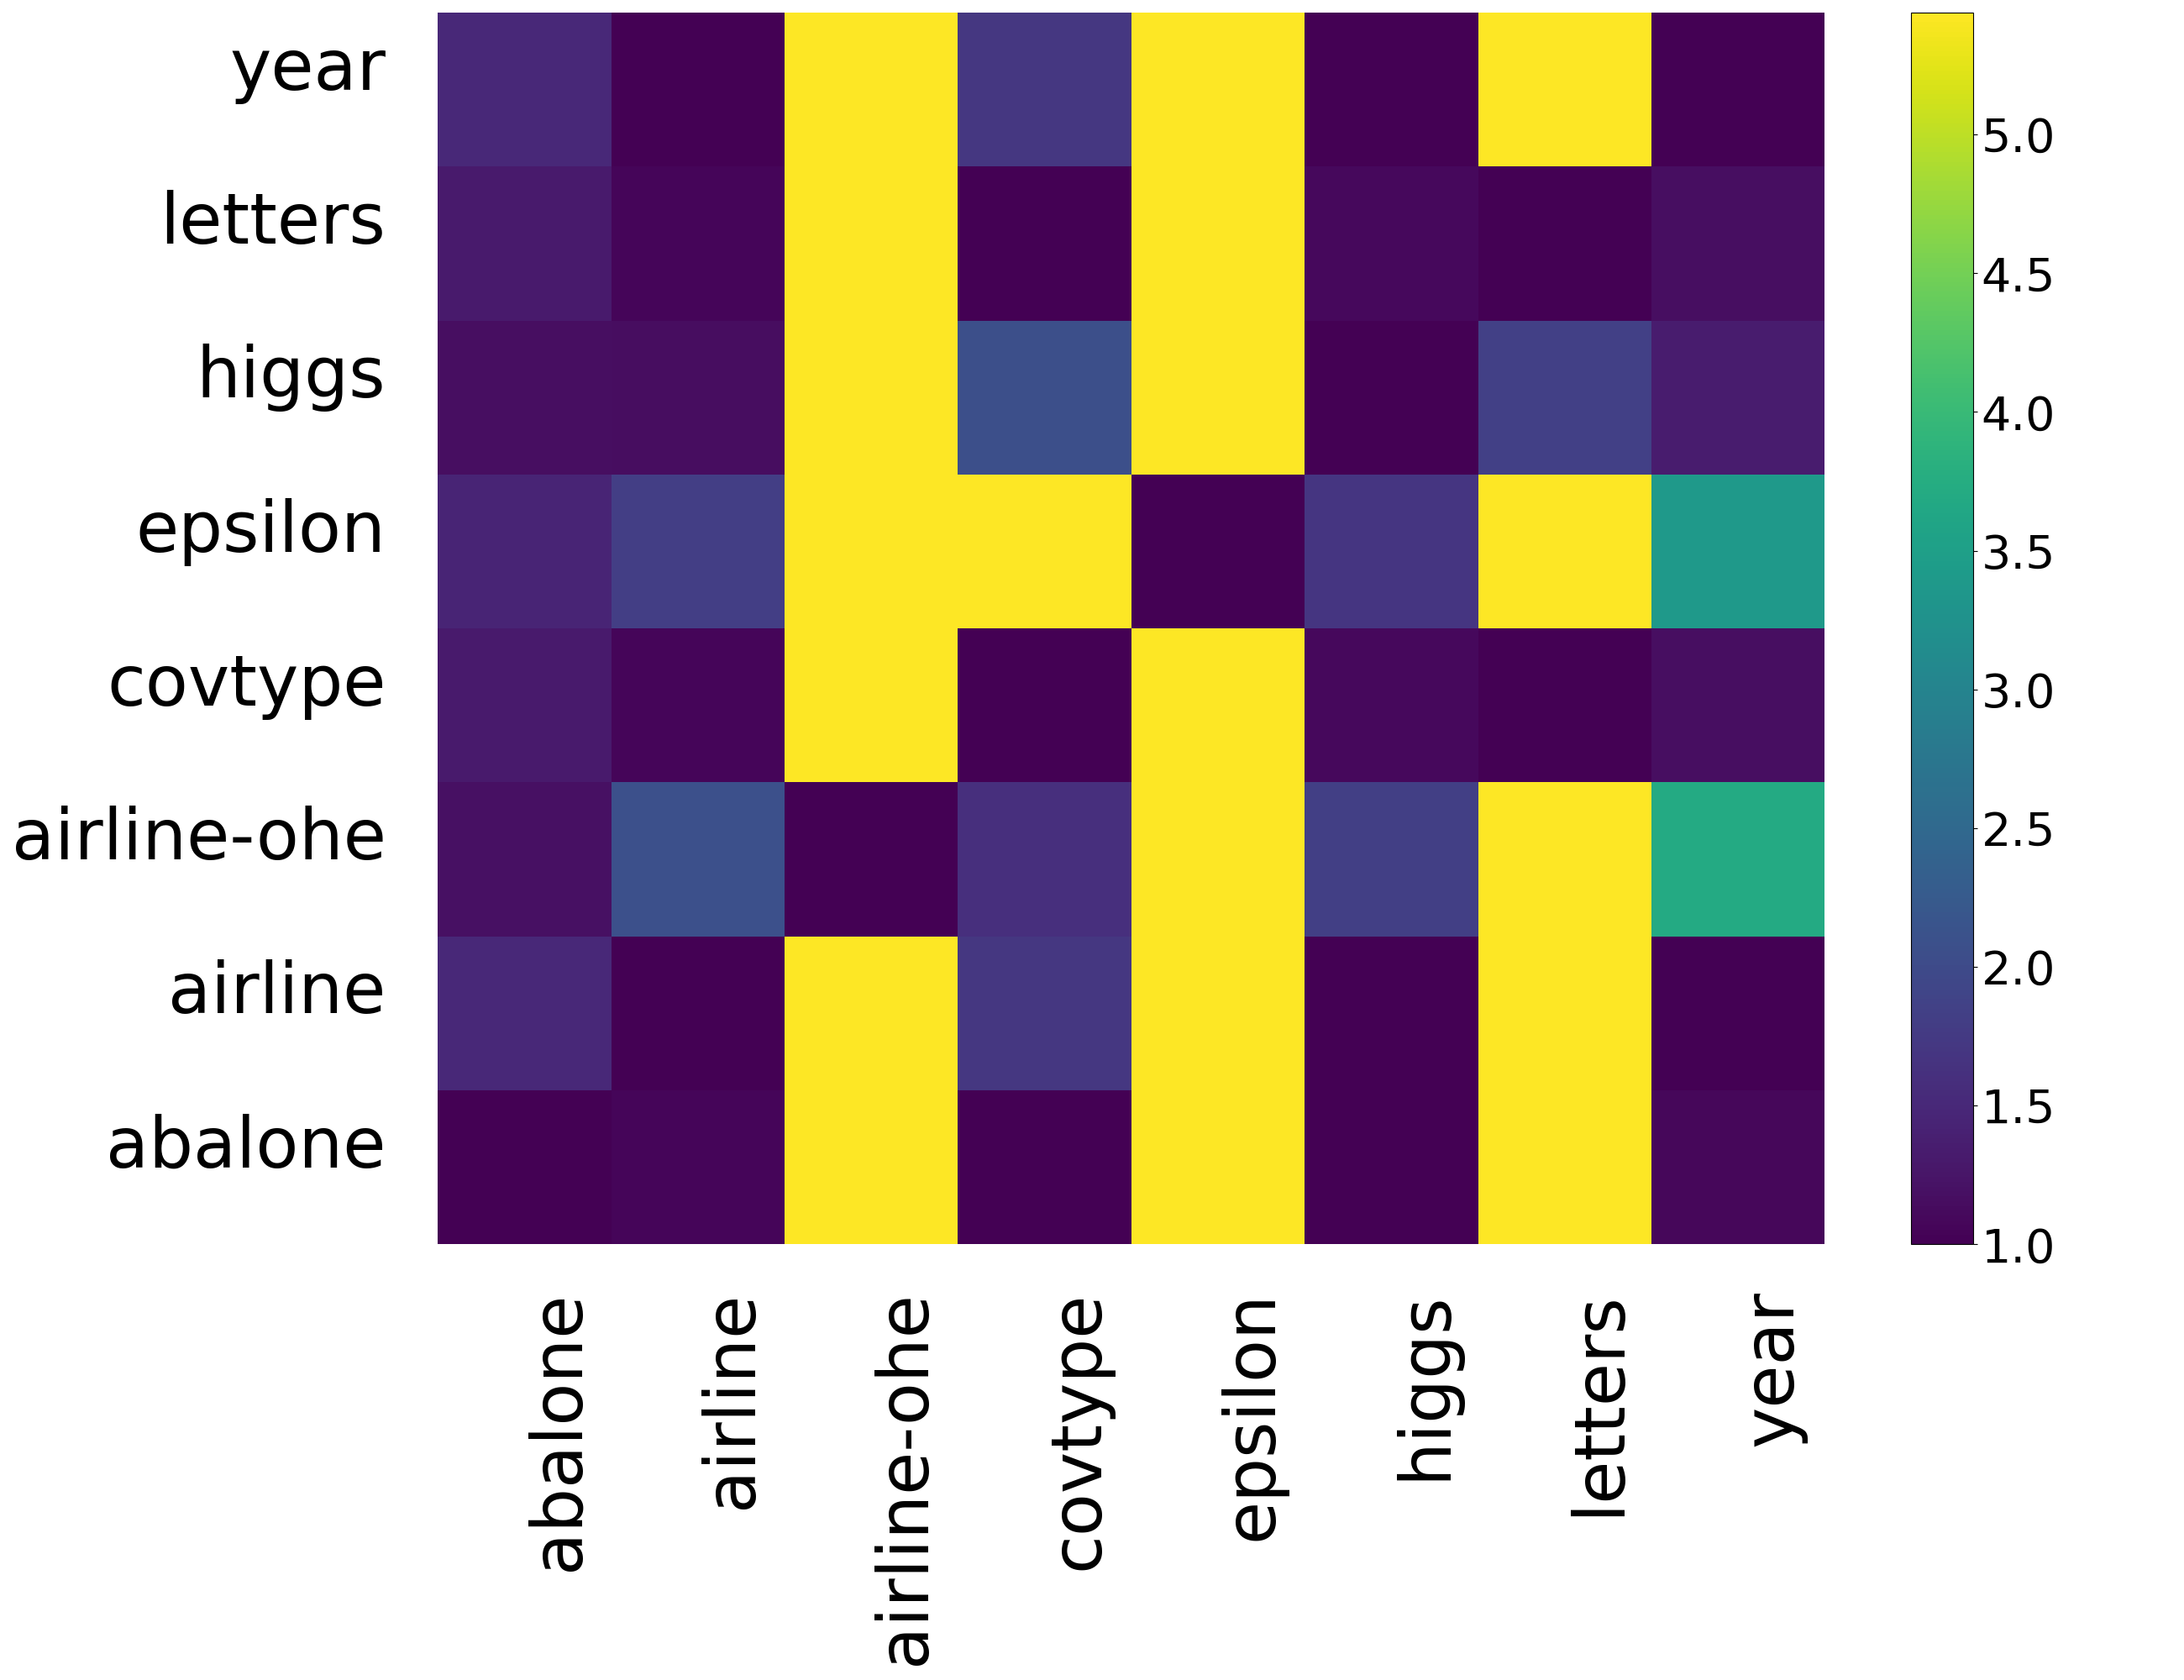
\includegraphics[width=\linewidth]{figures/model_sensitivity_4096.png}}
%     \caption{\label{fig:sensitivityb}Model sensitivity at batch size 4096}
%   \end{minipage}
%   \caption{Batch and model sensitivity plots. Each point shows the slowdown when best schedule for the
%           x-axis batch size (model) is used for the y-axis batch size (model).}
% \end{figure}

To establish the importance of choosing the right schedule, we
compare the performance of the schedules generated by \Treebeard{}
on several real-world benchmarks. 
Figure~\ref{fig:sensitivitya} shows the
variation in performance when the best schedule for a given batch 
size is used across different batch sizes for one of the models. 
Figure~\ref{fig:sensitivityb} shows the variation when schedules 
are used across models at a fixed batch size.
% These diagrams show that the best schedules to use vary across batch sizes and models. 
As can be seen, performance degrades by 2$\times$ when the best schedule for a
smaller batch size is used for a larger batch size and vice-versa.
Across all our benchmarks, the largest slowdown is 5$\times$.  %% and 
The degradation is much worse when schedules are used across different models.
In many (\~20\%) instances, using the best schedule for one model 
to compile another results in a 5$\times$ slowdown.
As we report in Section \ref{sec:results}, reusing schedules across
different architecture also leads to significant slowdowns.
Clearly, using a single strategy across models, batch sizes and targets
leaves significant performance on the table. 

These performance considerations, coupled with 
the importance of running ML applications on a diverse set of hardware targets,
motivates the need for a retargetable compiler for decision tree inference.
Building such a configurable compiler and supporting code generation for CPUs and GPUs 
required us to solve several fundamental problems. 
% We had to enable the
% compiler to represent and optimize reductions, deal uniformly with different
% in-memory representations of the model, design optimizations to effectively 
% use the memory hierarchy of the target processor (shared memory on GPUs and 
% cache on the CPU) and finally be able to generate target specific code. 
% %% RG
% Lastly, we propose a simple heuristic to find a high-performance schedule 
% for a given model and batch size to remove this burden from the user. 
% We defer the task of implementing an auto-tuner to future work. 
% %%
The rest of the paper describes these challenges in detail and how we
solved them in \Treebeard{}.

% Our main aim while designing \Treebeard{} was to unify the diverse set of implementation
% strategies that have been used in existing systems for decision tree inference. Some 
% differences in these systems are as follows:
% \begin{itemize}
%   \item Decision tree inference is run on several platforms including CPUs and GPUs. The 
%   implementations used on each of these platforms are different and the techniques used
%   to optimize them are also different.
%   \item A diverse set techniques have been proposed for optimization of decision tree 
%   inference on CPUs and GPUs \cite{VPred, Tahoe, Treelite, XGBoost, Hummingbird, QuickScorer, FIL}. 
%   No system exists that unifies the disparate optimizations implemented in these systems.
%   \item A very extensive design space of optimizations exists for decision tree inference
%   outside the few that have been proposed in the literature. However, currently no 
%   system exists that is capable of exploring this space and identifying the best set 
%   of parameters to use for a given model and platform.
%   \item Different systems use different in-memory representations for the model. For example,
%   XGBoost uses a sparse representation, RAPIDs FIL uses what is called the reorg representation 
%   and Tahoe uses a variation of the reorg representation. Currently, systems implement 
%   inference kernels that are tied to a single representation of the model. Again, this means
%   that no current system can explore different combinations of in-memory representations 
%   and optimizations.
% \end{itemize}
% At high-level, to make \Treebeard{} capable of unifying these differences, we design 1)  
% expressive intermediate representations that can represent and compose several proposed 
% optimizations 2) a scheduling language that specifies the structure of the
% generated code and 3) a plugin mechanism with which different in-memory representations
% can be composed with different optimizations. Finally, we develop a heuristic to
% explore the extensive optimization space that \Treebeard{}'s design enables.

% While a diverse set techniques have been proposed for optimization of decision tree 
% inference on CPUs and GPUs \cite{VPred, Tahoe, Treelite, XGBoost, Hummingbird, QuickScorer, FIL},
% a very extensive design space of optimizations exists 
% outside what has been proposed in the literature. Furthermore, decision tree inference 
% is run on several platforms including CPUs and GPUs. The implementations used on each of 
% these platforms are different and the techniques used to optimize them are different.
% To make matters even more complicated, several in-memory representations
% have been proposed for decision tree models. For example, XGBoost\cite{XGBoost} uses a sparse representation,
% RAPIDs FIL\cite{FIL} uses what is called the reorg representation and Tahoe uses a variation of the reorg
% representation. 
% \TODO{Can we add some numbers here to show that different models/batch sizes need different optimizations?}

% To solve the problems of exploring the design space of optimizations for decision tree
% inference and enabling portable performance, we build several techniques in \Treebeard{}, 
% an open source compiler infrastructure for decision tree inference. To make \Treebeard{}
% capable of unifying these different techniques and targets, we do the following. 
% \begin{itemize}
%   \item We design a scheduling language that encapsulates various optimization techniques
%   and controls the structure of the generated code.
%   \item We design an MLIR dialect to represent and optimize reductions and use this 
%   dialect within \Treebeard{} to enable the generation of different variants of 
%   inference routines.
%   \item We extend \Treebeard{}'s intermediate representations to include operations like caching.
%   We were able to easily reuse and extend \Treebeard{}'s IR as it was built as an MLIR dialect.
%   \item We design a plugin mechanism with which different in-memory representations
%   can be composed with different optimizations.  
% \end{itemize}
